
\section{Ancient DNA}

You are hiking on the Pyrenees mountain range and you discovered an ancient human bone.
You extracted the DNA and sequenced its genome.
Unfortunately the sample was not well preserved and it was highly contaminated.
Therefore you were able to obtain the genotypic information for only one locus.
Specifically, you found that, at a specific genomic position, the mysterious ancient human has an \texttt{AA} genotype, homozygous for adenine.
Nevertheless, you want to make some statistical inferences on whether this sample is genetically closer to modern Spanish, French or Basque individuals.
This analysis is a proxy for understanding whether this sample is more likely to be an ancestor for modern Spanish, French or Basque.
In other words, you want to perform a \textbf{population assignment} based on genetic data.

Let's assume that your parameter of interest is $\theta=\{S,F,B\}$ representing the probability that your sample comes from a Spanish (S), French (F) or Basque (B) population, respectively.
The data is $y=\{g, f_A^{(S)}, f_A^{(F)}, f_A^{(B)}\}$ where $g$ is the ancient genotype (so that $g=AA$) and $f_A^{(S)}$, $f_A^{(F)}$, $f_A^{(B)}$ are the known population frequencies of allele $A$ in modern Spanish, French and Basque, respectively.
Under the assumption of Hardy Weinberg Equilibrium, we know that
\begin{equation*}
p(g=AA, f_A^{(i)}|\theta=i)=(f_A^{(i)})^2
\end{equation*}
for a generic population $i$.
Note the latter equation represents the likelihood function $f(y|\theta)$.

\paragraph{Question A}

Using Bayes' law, write the equation for the posterior probability of the sample belonging to the Spanish population given the data. Assume that you have a generic prior probability $\pi(\theta)$ with known hyperparameters. Be as formal and explicit as possible. No proofs or extra calculations are required.
Let's assume that we gather the follow population allele frequencies
\begin{align*}
f_A^{(S)} &= 0.7\\
f_A^{(F)} &= 0.2\\
f_A^{(B)} &= 0.1\\
\end{align*}
and that we ask for an opinion to experts regarding a prior probability of this sample belonging to any of the tested populations.
Here the opinion from our 3 experts:
\begin{enumerate}
        \item Dr Cobain: \texttt{It is still highly debated whether ancient humans in the Pyrenees are the ancestors of modern French, Spanish or Basque. All anthropological evidences so far are not solid enough to point towards any specific population. We have no clue!}
    \item Professor Grohl FRS: \texttt{It must be Spanish. I see no evidence why this sample should be the ancestor of any other modern population. I am 100\% sure.}
    \item Mr Novoselic: \texttt{We have collected more than 1,000 ancient samples from Pyrenees so far and we were able to assign 50\% of them as Spanish, 30\% as French, and 20\% as Basque.}
\end{enumerate}

\paragraph{Question B}

Based on this information, choose the most suitable prior distribution $\pi(\theta)$. Justify your choice. There is no right or wrong answer (although one of them is hardly acceptable) as long as it is properly justified. Formalise $\pi(\theta)$ by assigning a prior probability for each value of $\theta$ based on your choice.

\paragraph{Question C}

Based on your chosen prior distribution, calculate the Bayes factor for model $M_1$ with parameter $\{\theta=S\}$ \textit{vs.} model $M_2$ with parameter $\{\theta \neq S\}$. Write the equation and provide the value for the Bayes factor. Approximate any calculation as much as you wish but be reasonable (e.g. $0.82/0.19 \approx 4$ is totally fine but $0.82/0.19 \approx 3$ is not). Provide a brief discussion on the support for $M_1$ or $M_2$.

\paragraph{Question D}

Let's assume that a new prior probability on $\theta$ is now dependent on an unknown hyperparameter $\tau$ with distribution $h(\tau)$ with $\tau=\{-1,0,1\}$. In other words, the prior distribution is $\pi(\theta|\tau)$ and $\tau$ can only have the discrete values of $-1$, $0$, or $-1$. Using Bayes' law in hierarchical modelling, write the equation for the posterior distribution of the sample being Spanish. Be as formal and explicit as possible. No proofs or extra calculations are required. Note that both $\theta$ and $\tau$ are discrete distributions.

Finally, you want to estimate the posterior distribution for the allele frequency of the ancestral Spanish population given the ancient and modern genotype data. Let's call this parameter $\phi$, continuous within the range $[0,1]$. The model is more complicated (and outside the scope of this exercise) and indeed you cannot derive a closed form for the posterior distribution. Therefore you want to use an indirect sampling method to approximate the posterior distribution $p(\phi|y)$.
As seen in class, one possibility is to use a \textit{rejection sampling} algorithm which uses an envelope function to "cover" the posterior distribution. However, this algorithm requires the specification of $M$ so that $L(\phi)\pi(\phi) < Mg(\phi)$ with $L(\phi)$ being the likelihood function. $M$ may be not readily available. Furthermore, this algorithm is computationally inefficient as it has a rejection step.

Therefore, you want to derive and implement a more efficient algorithm for indirect sampling of the posterior distribution, $p(\phi)$. Suppose you have $N$ draws of $\phi$ (so $\phi_1$, $\phi_2$, ...$\phi_N$) sampled from some approximating density function $g(\phi)$. This situation is illustrated in Figure \ref{fig:approx}. The continuous black line is the unknown posterior distribution, or a distribution up to a constant to $L(\phi)\pi(\phi)$; the red dashed line is the chosen approximating density $g(\phi)$; red small vertical lines on the x-axis represent the $N$ samples drawn which are then evaluated at $g(\phi)$.

\begin{figure}[h!]
        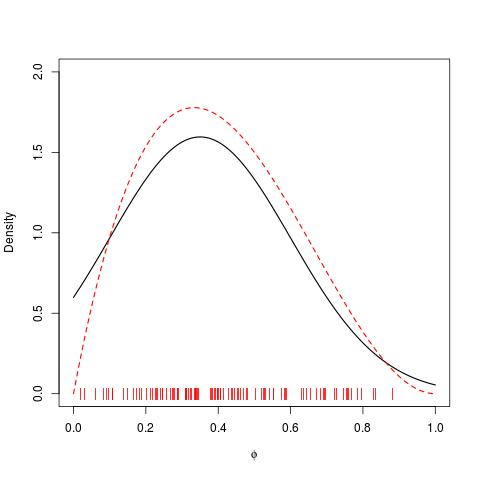
\includegraphics[width=0.9\textwidth]{Figures/sampling.jpeg}
	\caption{Indirect sampling to approximate a posterior distribution.}
    \label{fig:approx}
\end{figure}

\paragraph{Question E}

Assume that you can evaluate $L(\phi_i)\pi(\phi_i)$ and $g(\phi_i)$ for each one of the $N$ draws of $\phi$. You cannot sample from $L(\phi)\pi(\phi)$ but you can sample from $g(\phi)$ which is an approximating function for the posterior distribution. Devise an efficient algorithm for sampling $\phi_i$ to approximate the posterior distribution. Discuss what happens when $N$ becomes larger and any potential limitation of this method (e.g. based on the choice of $g(\phi)$).

(Hint: If $g(\phi) \equiv p(\phi|y)$ then your sample $\phi_1$, $\phi_2$, ...$\phi_N$ is already a sample from posterior. However, since $g(\phi)$ is just an approximating function, you do not want to resample from the set $\{\phi_1, \phi_2, ...\phi_N\}$ with equally likely probability of selection... )


